% EE Thesis/Dissertation
% Please see http://ee.tamu.edu/~tex for information about EE Thesis.

\documentclass[a4paper]{aitthesis}


\RequirePackage[sectionbib,round]{natbib}
\bibliographystyle{apalike}
\usepackage{siunitx}
\usepackage{enumitem} 
\usepackage[section]{placeins}
\usepackage{tcolorbox}
\usepackage{longtable}
\usepackage{acro}
\RequirePackage[hyphens]{url}
\RequirePackage[pagebackref]{hyperref}
\renewcommand{\backref}[1]{[p#1]}

% Dark blue colour for all links
\RequirePackage{color}
\definecolor{link}{rgb}{0.45,0.51,0.67}
\hypersetup{
  colorlinks,%
  citecolor=link,%
  filecolor=link,%
  linkcolor=link,%
  urlcolor=link,
}
\usepackage{graphicx}
\usepackage{amssymb,amsthm,amsmath}
\renewcommand{\listfigurename}{LIST OF FIGURES}
\renewcommand{\listtablename}{LIST OF TABLES}
\renewcommand{\contentsname}{LIST OF CONTENTS}

\acsetup{make-links, list/template= longtable}
\usepackage{verbatim}
\usepackage{multirow}   
\usepackage{bm}
\usepackage{url}
\usepackage{algorithm}
\usepackage{algcompatible}
\usepackage{placeins}
\usepackage{times}
\usepackage{array}
\usepackage[caption=false,font=footnotesize]{subfig}
\usepackage{tikz}

\DeclareAcronym{fkv}{
  short=FKV,
  long=formalin killed vaccines,
}
\DeclareAcronym{gbs}{
  short=GBS,
  long=Group B streptococci,
}
\DeclareAcronym{hrp}{
  short=HRP,
  long=horseradish peroxidase,
}
\DeclareAcronym{gp}{
  short=GP,
  long=Gram-positive,
}
\DeclareAcronym{mic}{
  short=MIC,
  long=Minimum inhibitory concentration,
}
\DeclareAcronym{s.}{
  short=S.,
  long=Streptococcus,
}
\DeclareAcronym{a.veronii}{
  short=\underline{\textit{A.veronii}},
  long=\underline{\textit{Aeromonas veronii}},
}
\DeclareAcronym{s.agalac}{
  short=\underline{\textit{S.agalactiae}},
  long=\underline{\textit{Streptococcus agalactiae}},
}
\DeclareAcronym{(v/v)}{
  short= \textit{\%(v/v)} ,
  long=Volume per volume (volume concentration of a solution),
}
\DeclareAcronym{tsb}{
  short=TSB,
  long=Tryptic soy broth,
}
\DeclareAcronym{bhi}{
  short=BHI,
  long=Brain heart infusion,
}
\DeclareAcronym{hkv}{
  short=HKV,
  long=Heat killed vaccines,
}
\DeclareAcronym{cfu}{
  short=CFU,
  long=Colony-forming units (CFU),
}
\DeclareAcronym{chitralada4}{
  short=Chitralada 4,
  long=Strain of Nile tilapia developped at Asian Institute of Technology,
}
\DeclareAcronym{saav}{
  short=Sa+Av,
  long=Bivalent vaccine against \underline{\textit{S.agalactiae}}+\underline{\textit{A.veronii}},
}
\DeclareAcronym{sa}{
  short=Sa,
  long=Vaccine against \underline{\textit{Streptococcus agalactiae}},
}
\DeclareAcronym{av}{
  short=Av,
  long=Vaccine against \underline{\textit{Aeromonas veronii}},
}
\DeclareAcronym{control}{
  short=Ct,
  long=Control 
}
\DeclareAcronym{onilo}{
  short=\underline{\textit{O.niloticus}},
  alt=\underline{\textit{Nile tilapia}},
  long=\underline{\textit{Oreochromis niloticus}},
}
\DeclareAcronym{wg}{
  short=WG,
  long=weight gain of the animals (in grams),
}
\DeclareAcronym{elisa}{
  short=ELISA,
  long=enzyme-linked immunosorbent assay,
}
\DeclareAcronym{ab}{
  short=Ab,
  long=antibodies,
}
\DeclareAcronym{ag}{
  short=Ag,
  long=antigenic particles or Antigens,
}
\DeclareAcronym{tsa}{
  short=TSA,
  long=tryptone soya agar,
}
\DeclareAcronym{sod}{
  short=SOD,
  long=superoxide dismutase,
}
\DeclareAcronym{cat}{
  short=CAT,
  long=catalase,
}
\DeclareAcronym{gpx}{
  short=GPx,
  long=glutathione peroxidase,
}
\DeclareAcronym{ros}{
  short=ROS,
  long=reactive oxygen species,
}
\DeclareAcronym{prrs}{
  short=PRRs,
  long=pathogen recognition receptors,
}
\DeclareAcronym{pamps}{
  short=PAMPs,
  long=pathogen-associated molecular patterns,
}
\DeclareAcronym{nos}{
  short=NOS,
  long=nitric oxide synthetase,
}
\DeclareAcronym{srt}{
  short=SRT,
  long=sex-reveral therapy,
}
\DeclareAcronym{ld50}{
  short=LD50,
  long=lethal dose able to terminate 50\% of a population,
}
\DeclareAcronym{ld100}{
  short=LD100,
  long=lethal dose able to kill 100\% of a population,
}
\DeclareAcronym{ip}{
  short=IP,
  long=intra peritoneal injection,
  alt=intra peritoneally injected,
}
\DeclareAcronym{dpv}{
  short=dpv,
  long=days post-vaccination,
}
\DeclareAcronym{pbs}{
  short=PBS,
  long=phosphate buffer saline,
}
\DeclareAcronym{igm}{
  short=IgM,
  long=immunoglobulins M,
}
\DeclareAcronym{igt}{
  short=IgT,
  long=immunoglobulins T,
}
\DeclareAcronym{ig}{
  short=Ig,
  long=immunoglobulin,
}
\DeclareAcronym{rtpcr}{
  short=RT-PCR,
  long=real-time reverse transcription polymerase chain reaction,
}


% \newcommand{\oops}[1]{\bf{#1}}
% \newcommand{\ga}{\bar{\gamma}}
% \newcommand{\myint}{\int_0^{\infty}}
% \renewcommand{\vec}[1]{\mathbf{#1}}
% \newcommand{\mat}[1]{\mathrm{#1}}
% 
% \newcommand{\vectornorm}[1]{\left|\left|#1\right|\right|}
% 
% \newcommand{\ten}[1]{\mathcal{#1}}
% \newcommand{\crossmat}[1]{\begin{bmatrix} #1 \end{bmatrix}_{\times}}
% \newcommand{\class}[1]{{\cal C}_{#1}}
% \def\Rset{\mathbb{R}}
% \def\Pset{\mathbb{P}}
% \DeclareMathOperator*{\argmax}{argmax}
% \DeclareMathOperator*{\argmin}{argmin}
% \DeclareMathOperator*{\sign}{sign}
% % \def\norm{\mbox{$\cal{N}$}}
% \newcommand\parms{\vec{\lambda}}
% \newcommand\oldparms{\parms^{\text{old}}}
% \newcommand{\mypm}{\mathbin{\smash{%
% \raisebox{0.35ex}{%
%             $\underset{\raisebox{0.5ex}{$\smash -$}}{\smash+}$%
%             }%
%         }%
%     }%
% }

\def\short{1}
% \renewcommand{\contentsname}{My nice list of contents}
% \renewcommand{\listfigurename}{My nice list of figures}
% \renewcommand{\listtablename}{My nice list of table}
\begin{document}
% \renewcommand\listfigurename{LIST OF FIGURES}
\pagenumbering{roman}
\pagestyle{plain}
%==========================================================
%======================  FRONT STUFF ======================
%==========================================================

%======================= Cover Page =======================
%\begin{document}
\newpage
\pagestyle{plain}
\pagenumbering{roman}
\setcounter{page}{0}
\setcounter{tocdepth}{3}
%\setlength{\footskip}{-15mm}
\setlength{\textheight}{230mm}
\setlength{\voffset}{10mm}
\vskip -5em

\begin{center}
{ 
  \singlespace \uppercase{\bf SYSTEMIC AND MUCOSAL IMMUNE RESPONSE OF NILE TILAPIA BROODSTOCK TO MONOVALENT AND BIVALENT VACCINES AGAINST BACTERIA STREPTOCOCCUS AGALACTIAE AND AEROMONAS VERONII} \par
}
\vskip 2em
{
  \lineskip 1.5em
  \begin{tabular}[t]{c} by\\ \\ QUENTIN ANDRES
  \end{tabular}\par
}
%\vskip 5.6em

\vskip 3.5em
\singlespace A thesis submitted in partial fulfillment of the
requirements for the degree of Master of Science in Aquaculture and Aquatic Resources Management

%	\vskip 5em
\vskip 0.5em
{
  \singlespace
  \begin{center}
    \begin{tabular}{rl}
      \\[-1em]
      Examination Committee: & Dr.\ Krishna R.Salin (Chairperson) \\[-0.8em]
                             & Dr.\ Ha Thanh Dong \#1 \\[-0.8em]
                             & Dr.\ YOUR COMMITTEE \#2 \\\\

% UNCOMMENT THE LINES BELOW IF YOU HAVE THE EXTERNAL EXAMINER.
%      External Examiner:     & Prof.\ YOUR EXTERNAL EXAMINER \\[-0.8em]
%                             & Dept.\ of Electrical and Computer Engineering \\[-0.8em]
%                             & McGill University, Canada \\\\
		
      Nationality:     & French \\[-0.8em]
      Previous Degree: & Bachelor of Molecular Biology, Microbiology
                             and Genetics
\\[-0.8em]
                       & 	University of Nice – Côte d’Azur
		Nice, France\\[-0.8em]
      \\
      Scholarship Donor: & None\\[-0.8em]
      \\
    \end{tabular}
  \end{center}

  \vskip 3.0em
  \centerline{}
  \vskip 2em
}
\end{center}
\begin{center}
  \singlespace Asian Institute of Technology\\ School of Environment, Resources and Development\\ Thailand\\ April 2022
\end{center}
\vfill

%====================== AUTHOR’S DECLARATION ======================
\newpage
\pagestyle{plain}
\onecolumn % Single-column.
\if@twoside\else\raggedbottom\fi % Ragged bottom unless twoside option.
\setlength{\footskip}{8mm}
\begin{center}
{
  \large \bf AUTHOR’S DECLARATION\\ \vskip 1em
}
\vskip 1em
\end{center}
\singlespace
\doublespace
\hspace{8.5mm}
\vspace{-1em}

I, Quentin ANDRES, declare that the research work carried out for this thesis was in accordance with the regulations of the Asian Institute of Technology. The work presented in it are my own and has been generated by me as the result of my own original research, and if external sources were used, such sources have been cited. It is original and has not been submitted to any other institution to obtain another degree or qualification. This is a true copy of the thesis, including final revisions.
\begin{center}
\vskip 0.5em
{
  \singlespace
\begin{center}
    \begin{tabular}{rl}
      \\[-1em]

\\Date: &  \\[-0.8em]

\\Name (in printed letters): & QUENTIN ANDRES\\[-0.8em]

\\Signature: & \\[-0.8em]

      \\
    \end{tabular}
  \end{center}
  \vskip 3.0em
  \centerline{}
  \vskip 2em
}
\end{center}

%====================== ACKNOWLEDGEMENTS ======================

\newpage
\pagestyle{plain}
\onecolumn % Single-column.
\if@twoside\else\raggedbottom\fi % Ragged bottom unless twoside option.
\setlength{\footskip}{8mm}
\begin{center}
{
  \large \bf ACKNOWLEDGMENTS\\ \vskip 1em
}
\vskip 1em
\end{center}
\singlespace
\doublespace
\hspace{8.5mm}
\vspace{-1em}

Type your acknowledgments here. This section is typically reserved for personal and professional dedications. You may also acknowledge your donor or funder here or include copyright acknowledgements of journals whose articles you have significantly incorporated in this thesis. Maintain one blank 1.5 line spacing between paragraphs.


[one page, maximum]
\phantomsection
\addcontentsline{toc}{section}{ACKNOWLEDGMENTS}

%====================== ABSTRACT ======================
\newpage
\pagestyle{plain}
\begingroup
\hypersetup{linkcolor=black}
% \renewcommand\listfigurename{LIST OF FIGURES}


\phantomsection
\addcontentsline{toc}{section}{ABSTRACT}
\onecolumn % Single-column.
\if@twoside\else\raggedbottom\fi % Ragged bottom unless twoside option.

\setlength{\footskip}{8mm}

\begin{center}
{\large \bf ABSTRACT \\ \vskip 1em}
\vskip 1em
\end{center}
\singlespace
\doublespace
\hspace{8.5mm}
\vspace{-1em}

Fighting bacterial infections inducing mass mortality in fish is a hot-topic research in the aquaculture industry in order to sustain its intensification. This research project aims to develop monovalent and bivalent vaccines against \ac{gbs} \acs{s.agalac} and against \ac{gp} \ac{a.veronii} for prophylaxis of \underline{\textit{Nile tilapia}} (\acs{onilo}) for which there is currently no vaccine available in Thailand.  In the present research, \acs{fkv} were produced by pathogen inactivation method: formalin 1\% - 3 \acs{(v/v)} is added to the virulent pathogenic solution. The objective of the study is to characterize a part of the immune response elicited in \aca{onilo} in response to vaccination. A total of $(\mathrm{n} = 400 juveniles)$ with an average mass of $(\mathrm{m} = X\si{\gram} \mypm X'\si{\gram})$ were stocked into experimental ponds/aquariums prior to the start of the experiments. The population was then divided into 4 groups according to experimental design. After verification that the fish were free of any disease, they were acclimated for about a week. Meanwhile our 2 virulent pathogenic bacteria have been recovered and amplified on appropriate medium and were used for the vaccine production but also stored for challenge test. As a first step, a total of 4 treatments were administrated to the fish in order to monitor a possible immunization: 1 \Ac{control} (a vaccine with no immunizing properties) & 3 formalin inactivated vaccines \ac{fkv} containing either antigenic particles of \ac{s.agalac} (monovalent \acs{sa}); \ac{a.veronii} (monovalent \acs{av}); \ac{s.agalac} + \ac{a.veronii} (bivalent \acs{saav} with a 1:1 ratio). In a second step, the fish immune response to vaccination (=immunogenicity and survivability) was determined by titrating agglutinating antibodies \Acs{ab} but also with \acs{elisa} assay which is more reliable method. Indeed, isotype determination of \Acs{ab} can allow to determine the concentrations of specific \ac{igm} and \ac{igt} for \textit{\ac{s.agalac}'s} polysaccharides and \ac{a.veronii}. In addition, gene transcription activity from before, during, and after the immunization (up to 70 \ac{dpv}) were determined by \acs{rtpcr} for \ac{igm} and \ac{igt} (active transcripts) corresponding to humoral immunity, and for \ac{sod}, \ac{cat}, \ac{gpx}, \ac{nos} (respiratory burst activity of phagocytes, \ac{ros} producing) corresponding to innate immunity. As a final step, a challenge test in vivo was carried out on the fish juveniles with the two bacteria. Fish were injected with \acf{control}+\ac{pbs} or were \aca{ip} a lethal dose of pathogen according to their prior vaccination.

\endgroup
\setlength{\parskip}{0pt} 
%======================= Table of Contents =========================
\newpage
\phantomsection
\tableofcontents
% Page 2 begins
% %===================== List of Tables ======================
\newpage
\phantomsection
\addcontentsline{toc}{section}{LIST OF TABLES}
\listoftables

%===================== List of Figures ======================
\newpage
\phantomsection
\addcontentsline{toc}{section}{LIST OF FIGURES}
\listoffigures
\phantomsection
%\clearpage     % \clearpage ends the page, and also dumps out all floats.
%\end{document} % Floats are things like tables and figures.

%\clearpage     % \clearpage ends the page, and also dumps out all floats.

% %\clearpage     % \clearpage ends the page, and also dumps out all floats.
% %\end{document} % Floats are things like tables and figures.

%\clearpage     % \clearpage ends the page, and also dumps out all floats.

\setlength{\parskip}{12pt}

\newpage
\phantomsection
\addcontentsline{toc}{section}{LIST OF ABREVIATIONS}
\printacronyms[name= {\large LIST OF ABREVIATIONS}]



\small

\pagenumbering{arabic}
\setlength{\headheight}{12pt}
\pagestyle{plain}

\setlength{\footskip}{8mm}

\chapter{INTRODUCTION}

\section{Background of the Study}

Previous outbreaks of \ac{s.agalac}\label{acro:s.agalac} and \ac{a.veronii} in \aca{onilo}, Oreochromis niloticus, were reported in Japan, Taiwan, and the United States. \ac{a.veronii} and \ac{s.agalac} are widespread pathogens of \aca{onilo} world-wide  and induce mass mortality of the fish in a few days. The two bacterial isolates used in this research are from Thailand, where the bacteria are present and create substantial economic losses for Thai aquaculture industry.

\section{Statement of the Problem}

In order to sustain an intensified and resilient Cichlids' aquaculture, many research units and private companies around the world are studying immune responses of fish to viral and bacterial infections and are experimenting with vaccines development. There is currently no existing vaccine against the \ac{s.agalac} and \ac{a.veronii}. Oil-based \ac{fkv} can be used as a prophylaxis treatment for aqua-cultured freshwater fish and this method is cost efficient and a viable alternative for the \aca{onilo} that has not yet been developed in Thailand. A combined vaccination with a bivalent vaccine is the most cost-effective solution.

\section{Hypothesis}

Previous literature has shown the possibility to develop monovalent and multivalent vaccines for fish such as Asian seabass using whole inactivated pathogens. Assumption that Asian seabass and \aca{onilo} share a similar physiology and similar dynamics in their response to \ac{ag} support the possibility of making a vaccine for the \aca{onilo}.

My second assumption is the feasibility of the \acs{fkv} vaccine production using low-cost method with pathogen inactivation using a chemical: formalin with concentration of 1\% - 3 \acs{(v/v)}, which would make the vaccines cost-efficient for farmers and medium sized farms. 

\section{Objectives of the research project} 

The objective of this research is to create new cost-effective vaccines in the Nile Tilapia against two fish pathogens \ac{s.agalac} and \ac{a.veronii}.

The three vaccines developed are in the table 1:

\addcontentsline{lot}{chapter}{Table 1 \hskip 3.55em Summary of the inactivated vaccines used in the study }
\begin{center} 
  \caption{\textbf{Table 1}
  \textwidth
  \begin{tabular}{ll}
    \ac{a.veronii} & \ac{av} \\
    \ac{s.agalac} & \ac{sa} \\
    \ac{s.agalac} + \ac{a.veronii} & \ac{saav} 
  \end{tabular}
\end{center}

The vaccines will be \aca{ip} (\ac{ip}) in order to understand the elicited systemic and mucosal immune response of \aca{onilo}. In addition, the efficiency of the monovalent formulations (\ac{sa},\ac{av}) is compared versus the bivalent formulation (\ac{saav}) will be compared with a challenge test.

\section{Risks and limitations}

\subsection{Access to laboratory facilities}

The experiments will be held and conducted at Asian Institute of Technology in the AARM department (stocking of fish and vaccination and challenge) and at SSRU laboratory facilities (\ac{elisa}, agglutination test, \ac{rtpcr}) and eventually at Mahidol Centex Shrimp.

\subsection{Safety of experiments}

Culture of the bacteria might not cause a risk to the wild fish and environment because all the experimentations will be made in closed and hermetic culture systems with compliance and respect of the strict biosecurity rules. 

\subsection{Risks in the schedule}

The main challenges and risks could be due to any delays related fish keeping and fish culture or due to problems in the bacterial culture or vaccine preparation. It could eventually lead to a delay in the realization of the research project.

\section{Organization of the research project}

\subsection{Project fundings}

The project funding will come from the support of the AIT Innovative research fund.

\subsection{Organization of the research project}

I have divided my work in work packages.

I organize the rest of this research thesis as follows.

I have broken down the project work in several phases as shown in Figure 1.

In Chapter \ref{ch:literature-review}, I describe the literature review.

In Chapter \ref{ch:methodology}, I propose my methodology for the experimental design, for the pond preparation, the fish feeding regime. But also for bacterial culture, vaccination, fish mucus swabs and blood sampling. For antibody agglutination titration, \ac{elisa}, \ac{rtpcr} and finally for the Challenge tests. 

In Chapter \ref{ch:results}, I present the experimental results.

Finally, in Chapter \ref{ch:conclusion}, I conclude my thesis.

\beginfigure
  \begin{center}
  \begin{flushleft}
  \caption{\textbf{Figure 1: Steps of the research project}} \\
  \end{flushleft}\\
  \\
  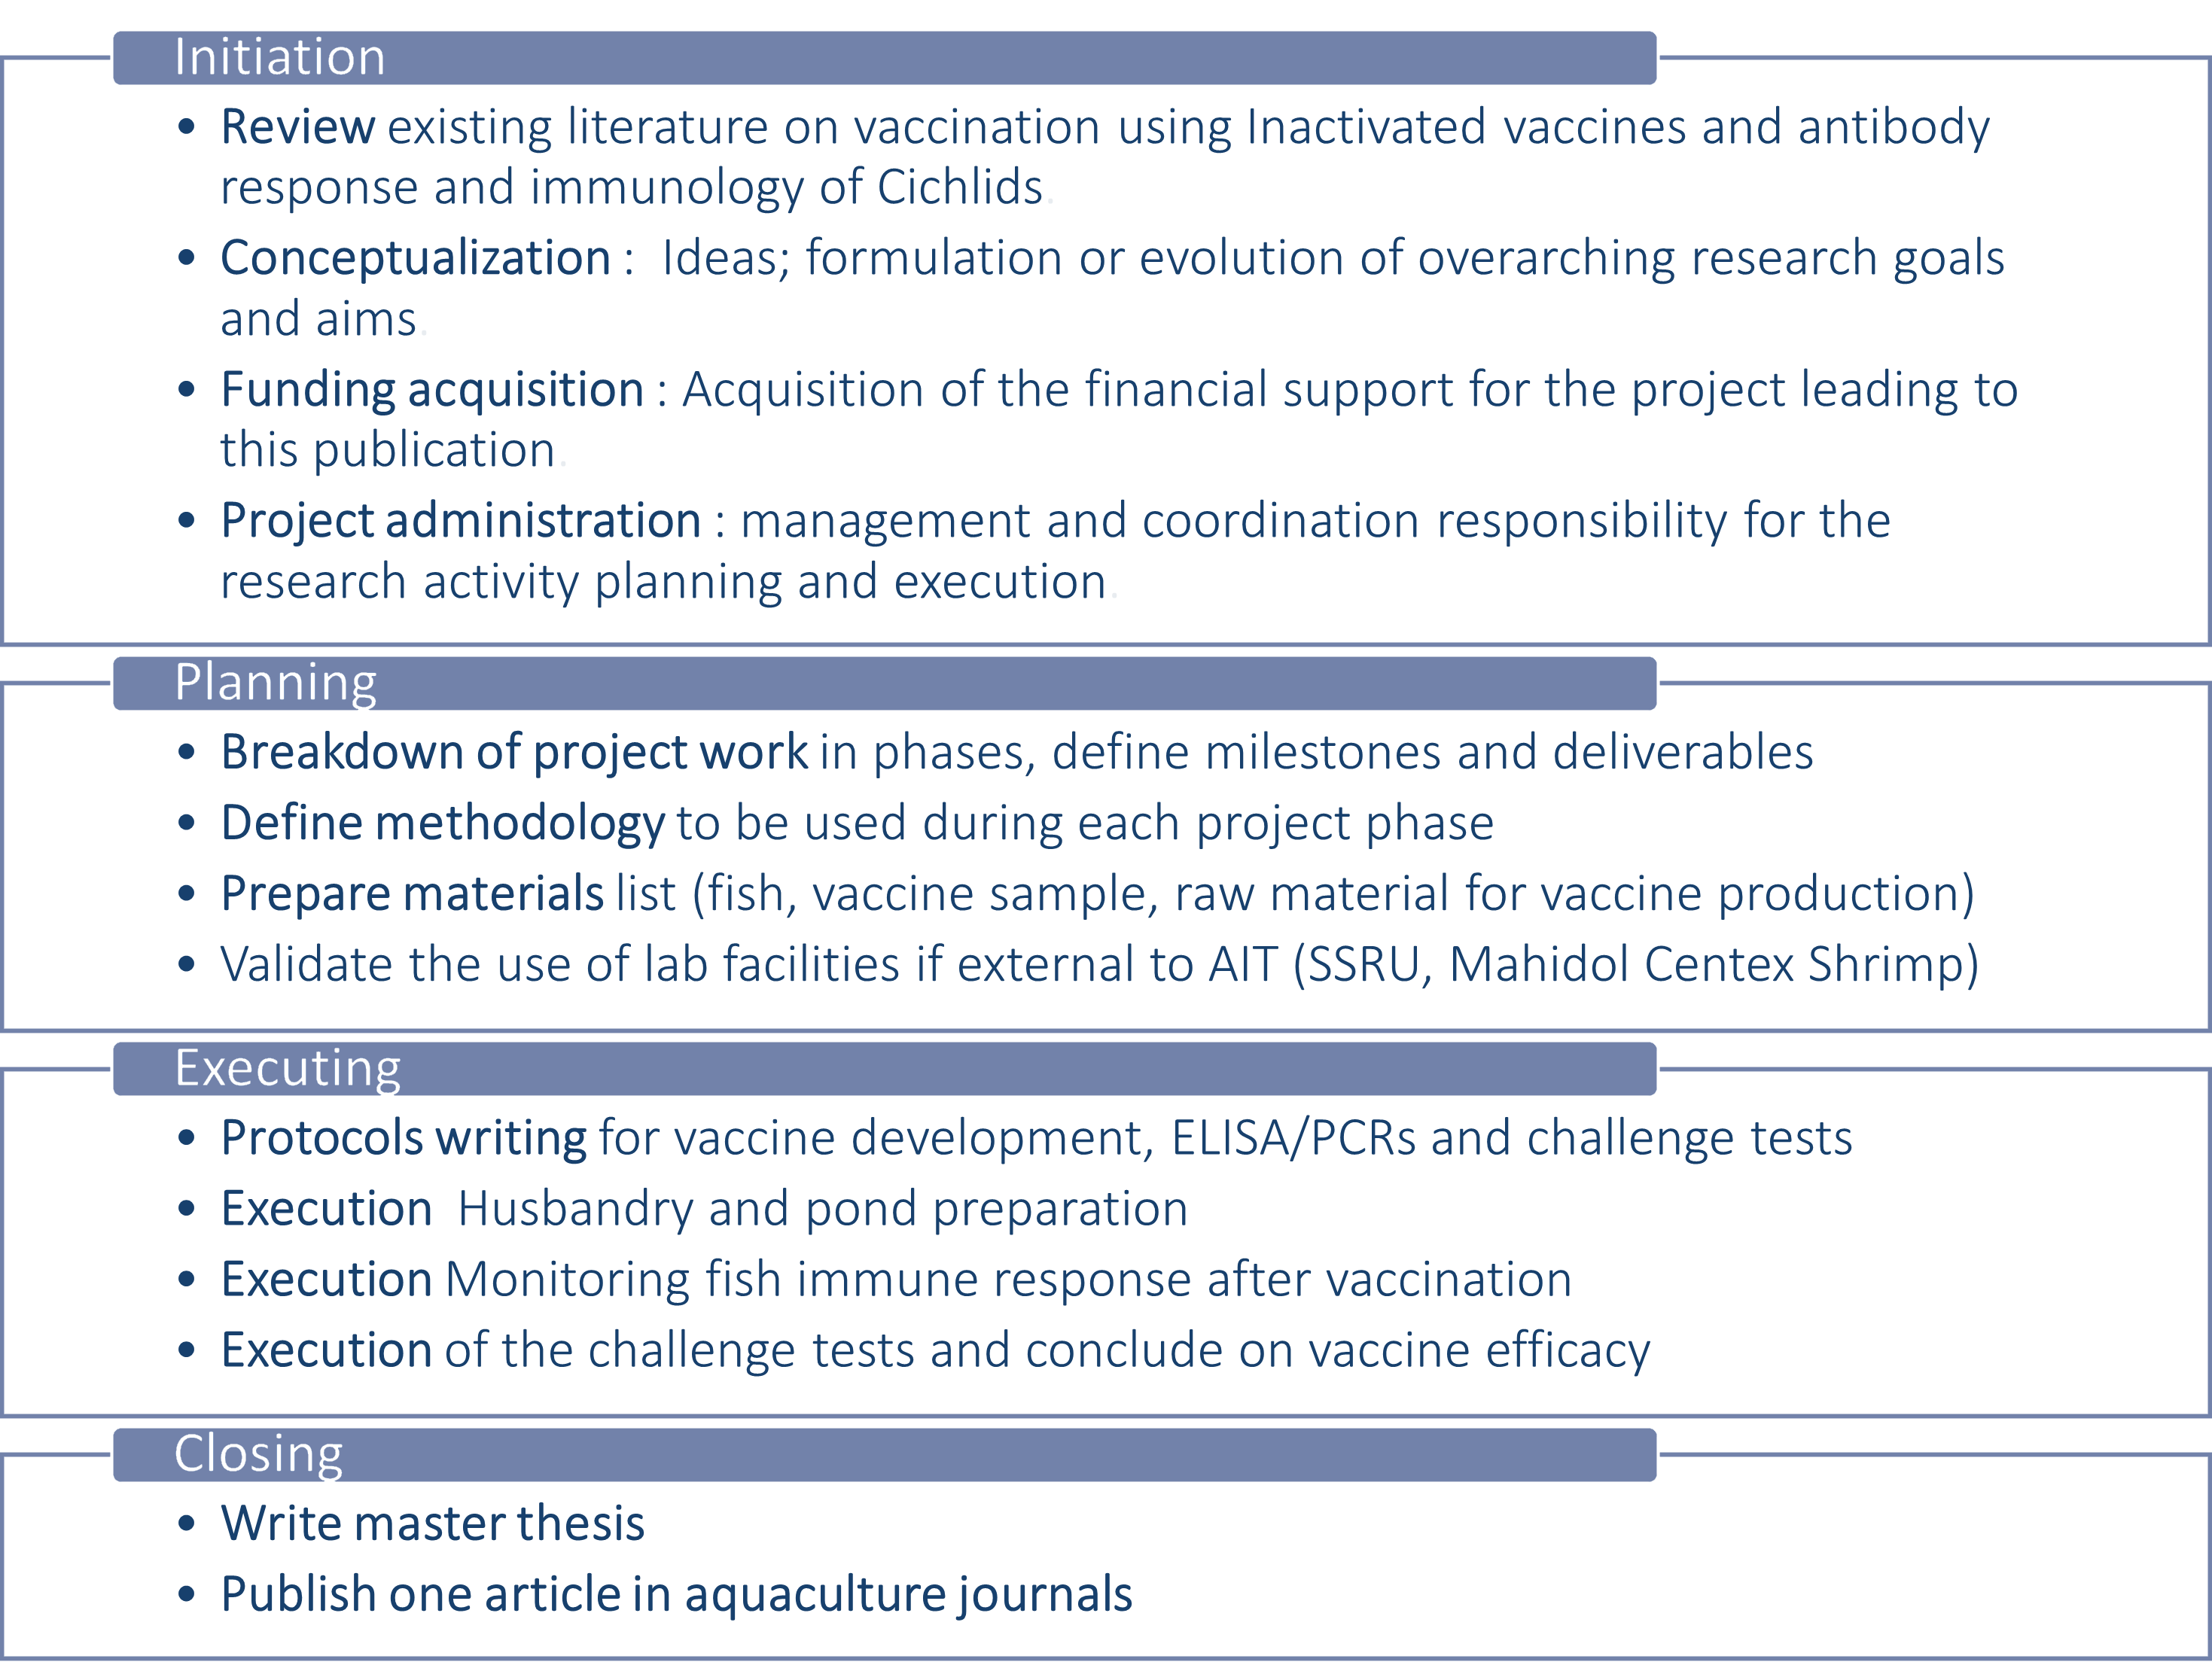
\includegraphics[width=\textwidth, height=\textheight, 
                 keepaspectratio]{figures/Figure1.png}
  \label{figure 1: The research plan}
  \addcontentsline{lof}{chapter}{Figure 1 \hskip 3.55em Organization of the research project}
  \endfigure
  \end{center}
\FloatBarrier

\pagestyle{plain}
\setlength{\footskip}{8mm}

\chapter{RELEVANT LITERATURE}
\label{ch:literature-review}

\textit{TO BE DONE LATER This chapter will provide a review of the relevant literature for which my project is based on.}

\section{Relevant literature on \ac{s.agalac} and \ac{a.veronii} and their infections in Nile tilapia} 

\subsection{\ac{s.agalac} pathogenesis}
\label{ssec:s-agalac-pathogenesis}

Some texts

\subsection{\ac{a.veronii} pathogenesis}
\label{ssec:a-veronii-pathogenesis}
\section{Relevant literature on whole pathogen inactivated vaccines} 
\label{sec:relevant-literature-on-whole-pathogen-inactivated-vaccines}

Some texts

\subsection{Formalin killed vaccines (\ac{fkv})}
\label{ssec:fkvs}

Some texts

\subsection{Heat killed vaccines (\acs{hkv})}
\label{ssec:hkvs}

Some texts

\newpage

\section{Relevant literature on systemic and mucosal fish immunology: Innate immunity} 
\label{sec:systemic-mucosal-immuno-innate}

Some texts

\subsection{Recognition of self and non-self, \aca{pamps} and \aca{prrs}}
\label{ssec:self-nonself-pamp-prr}

Some texts

\subsection{The complement system}
\label{ssec:complement}

Some texts

\subsection{Neutrophils}
\label{ssec:neutrophil}

Some texts

\subsection{Phagocytosis}
\label{ssec:phagocytosis}

Some texts

\subsection{Oxygenic respiratory burst}
\label{ssec:oxygenic-respiratory-burst}

Some texts

\newpage

\section{Relevant literature on systemic and mucosal fish immunology: Specific immunity}
\label{sec:systemic-mucosal-immuno-specific}

Some texts

\subsection{Immunoglobulins in fish}
\label{ssec:immunoglobulins-fish}

Some texts

\subsection{T cells and B cells}
\label{ssec:tcell-bcell}

Some texts

\newpage

\section{Relevant literature on antibody agglutination titration, ELISA (humoral immune system)} 
\label{sec:agglutination-elisa}

Some texts

\subsection{Antibody agglutination test}
\label{ssec:agglutination}

Some texts

\subsection{Enzyme-linked immunosorbent assay (\ac{elisa})}
\label{ssec:elisa}

Some texts

\newpage

\section{Relevant literature on leucocytes count and quantification of respiratory burst activation (innate immune system)}
\label{sec:leucocytes-respiratory-burst-activation}

Some texts

\subsection{Leucocyte cell count and haemodynamic parameters in fish.}
\label{ssec:leucocyte-count-heamodynamic-parameters}

Some texts

\subsection{Assays for the mesurement of the respiratory burst (reactive oxygen species \ac{ros}) and phagocytosis activity.}
\label{ssec:ROS-measurement-colorimetrie}

Some texts

\section{Chapter Summary}

Some texts

% THE REASON ~ IS USED HERE BECAUSE WE TELL LATEX THAT THESE TWO WORDS SHOULD 
% GO TOGETHER IN THE SAME LINE.

\FloatBarrier


\setlength{\footskip}{8mm}

\chapter{METHODOLOGY AND RAW MATERIAL}
\label{ch:methodology}


\textit{Some intro..}

\section{Project steps overview}

I will describe in the next paragraphs the methodology I will use for each of the steps described in Figure 3. TO BE CONTINUED

\section{Experimental design and statistical power analysis}


\addcontentsline{lot}{chapter}{Table 2 \hskip 3.55em Description of the experimental design}
\begin{center} 
  \begin{flushleft}
  \textwidth
  \addcontentsline{lot}{chapter}{Table 2.1 \hskip 3.55em Informations about animals and their origins}
  \caption{\textbf{Table 2.1 } \\
  ~ \\
  \subcaption{\textit{Informations about animals and their origins} \\
  ~ \\
  \end{flushleft} 
  \textwidth
  \begin{tabular}{ll}
    Fish population $(\mathrm{n} = 400 juveniles)$. \\
    Species = \ac{onilo}. \\
    Age = \textit{juveniles}. \\  
    Average mass of $(\mathrm{m} = X\si{\gram} \mypm X'\si{\gram})$. \\
    Secondary sexual gender: \textbf{ 100\% underwent \ac{srt}}. \\
    Origin = \textbf{Thailand}, Asian institute of technology. \\
    Strain = \textbf{Chitralada 4}. \\
    Pathogen free = \textbf{required}. \\
  \end{tabular}
\end{center}

\textbf{Detection of diseases (procedure):} Select \textbf{6-10} individuals at random, kill them, culture brain and head kidney on \ac{tsb} for detection of pathogens (\ac{a.veronii} and \ac{s.agalac}). \\

\textbf{How many groups for the vaccination?}  Create \textbf{4} groups/subsets of approx. \textbf{100-150} individuals. \\
    \textbf{4} ponds/aquariums for \textbf{10} days(Acclimatation) + \textbf{70} days(post vaccination) = \textbf{80} days. \\
  
\textbf{Methodology for flood and mucus sampling:} Select not less than \textbf{8} fish per group for \textbf{blood} and \textbf{mucus} swab every week. \\

\textbf{Challenge test:} Separate the fish in 2 sub-groups for \ac{control}, \ac{av} \textbf{monovalent}, \ac{sa} \textbf{monovalent}. In 3 sub-groups for \ac{saav} \textbf{bivalent}, as indicated below: \\
\newpage

\begin{center}
  \caption{\textbf{Table 2.2 Summary of the different groups getting vaccinated}. \\
  \\
   \begin{flushleft}
  \textwidth
  \addcontentsline{lot}{chapter}{Table 2.2 \hskip 3.55em Summary of the different groups getting vaccinated}
  \caption{\textbf{Table 2.2 } \\
  ~ \\
  \subcaption{\textit{Summary of the different groups getting vaccinated} \\
  ~ \\
  \end{flushleft} 
  \textwidth
  \begin{tabular}{ll}
    \textbf{Control} (sham vaccinated) challenged with \ac{s.agalac} = \textbf{33} fish. \\
    \textbf{Control} (sham vaccinated) challenged with \ac{a.veronii} = \textbf{33} fish. \\
    \textbf{Control} (sham vaccinated) challenged with \ac{pbs} = \textbf{33} fish. \\
    \ac{sa} \textbf{monovalent} challenged with \ac{s.agalac} = \textbf{50} fish. \\
    \ac{sa} \textbf{monovalent} challenged with \ac{pbs} = \textbf{50} fish. \\
    \ac{av} \textbf{monovalent} challenged with \ac{a.veronii} = \textbf{50} fish. \\
    \ac{av} \textbf{monovalent} challenged with \ac{pbs} = \textbf{50} fish. \\
    \ac{saav} \textbf{bivalent} challenged with \ac{s.agalac} = \textbf{33} fish. \\
    \ac{saav} \textbf{bivalent} challenged with \ac{a.veronii} = \textbf{33} fish. \\
    \ac{saav} \textbf{bivalent} challenged with \ac{pbs} = \textbf{33} fish. \\
  \end{tabular}
\end{center}
    
\textbf{Statistical power analysis:}  It is possible to create an artificial population of each group composed of 20 000 sampling with replacement and use the Central limit theorem to deduce the Standard error of the means and infer our vaccine efficiency for all the juveniles Chitralada 4 in the world (main population) with 95\% confidence using an approximation of the Standard deviation.

\section{Methodology for pond preparation and fish stocking}

\newpage

\section{Methodology for bacterial culture and bacterial preparation}

\beginfigure
  \begin{center}
  \begin{flushleft}
  \caption{\textbf{Figure 3: Schema of an antibiogram}}
  \end{flushleft} \\
  \\
  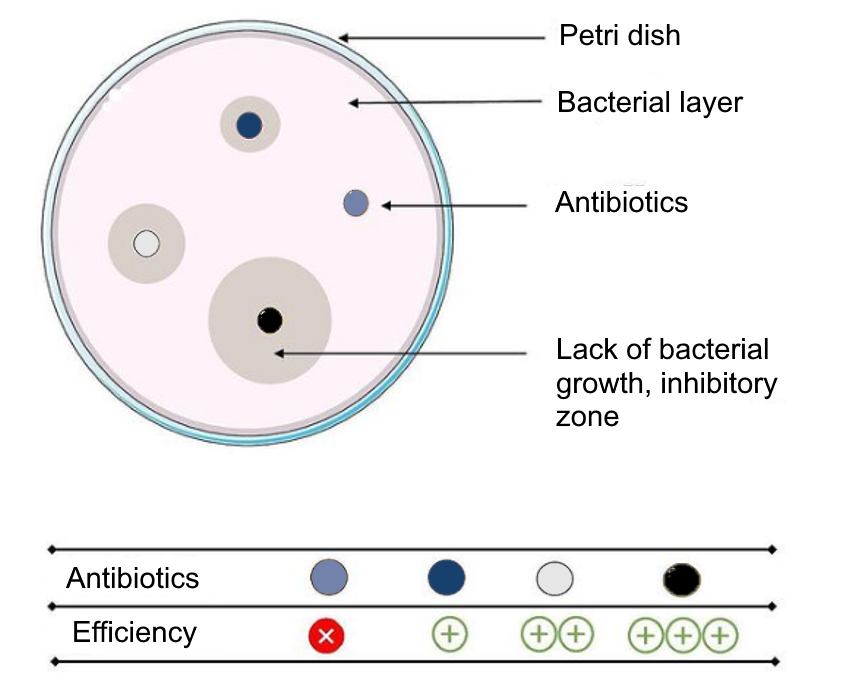
\includegraphics[width=0.8\textwidth, height=0.8\textheight, 
                 keepaspectratio]{figures/Figure3a.png}
  \label{Figure 3: Schema of an antibiogram (general principle)}
  \addcontentsline{lof}{chapter}{Figure 3 \hskip 3.55em Schema of an antibiogram (general principle)}
  \endfigure
  \end{center}


\subsection{For \ac{s.agalac}}

Antibiogram \ac{s.agalac}: 

\subsection{For \ac{a.veronii}}

Antibiogram \ac{a.veronii}: 


\section{Methodology for preparation of formalin killed vaccines (FKVs)}

Volume to inject  ${100\si{\micro\liter}\ac{ip} / fish}$

\section{Methodology for vaccine administration in fish and monitoring of fish health during bacterial challenge test}

\section{Methodology for fish sera and mucus extraction}

\section{Methodology for \ac{elisa} assays for specific \ac{igm}, \ac{igt} titrations}

\ac{elisa} is an enzyme-linked immunosorbent assay "for the presence of antibodies, antigens", proteins and glycoproteins in biological samples. \ac{elisa} technique is widely used for rapid diagnostic tests such as the diagnosis of HIV infection, pregnancy tests or the detection of food allergens.

The principle of this technique is based on the use of an enzyme conjugated to an antibody which by reacting with a colorless substrate gives a colored reaction product and which is therefore detectable. This is called a chromogenic substrate. Different enzymes are used for \ac{elisa} tests including alkaline phosphatase, \ac{hrp} or beta-galactosidase.

The \ac{elisa} assay will give information on the \ac{ab} titer of the fish, \ac{igm} and \ac{igt} respectively will be targeted in the assay.

\section{Methodology for \ac{rtpcr}}

The reference genes for the \ac{rtpcr} of \ac{onilo} are genes ubiquitously and constitutively expressed in the animal. They are also well known as "house-keeping" genes/mRNAs. (see below). 

\beginfigure
  \begin{center}
  \begin{flushleft}
  \caption{\textbf{Figure 4: Reference genes used in RT-PCR technique for Tilapia}
  \subcaption{\textit{Credits:\url{http://dx.doi.org/10.1016/j.gene.2013.06.013}}}
  \end{flushleft} \\
  \\
  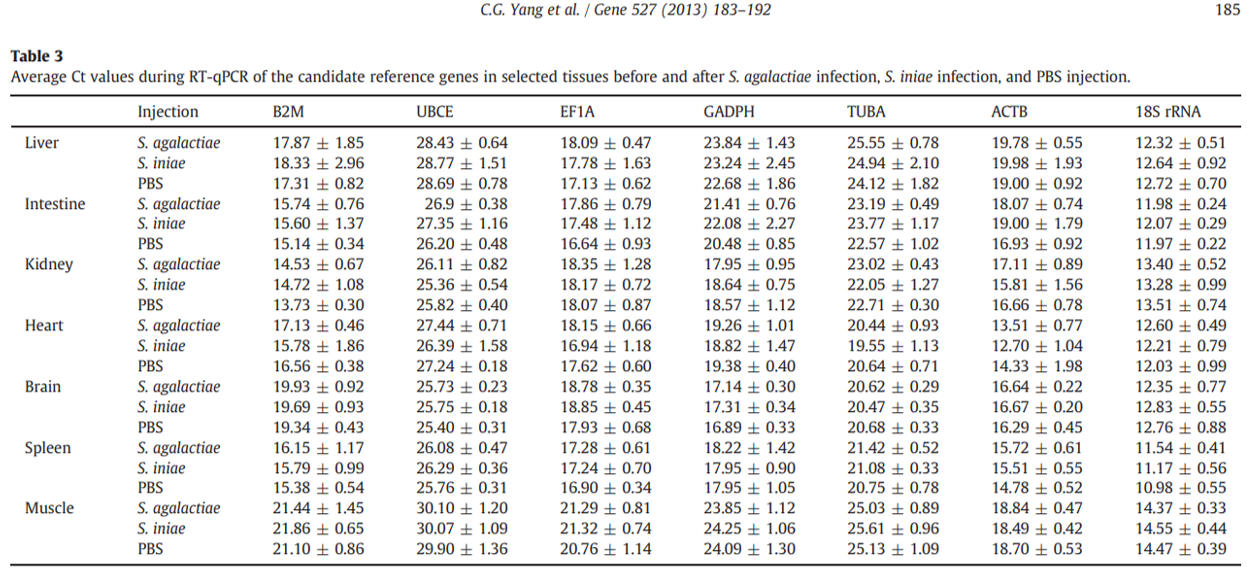
\includegraphics[width=\textwidth, height=\textheight, 
                 keepaspectratio]{figures/FigurePCR.png}
  \label{Reference genes used in RT-PCR technique for Tilapia}
  \addcontentsline{lof}{chapter}{Figure 4 \hskip 3.55em Reference genes used in RT-PCR technique for Tilapia}
  \endfigure
  \end{center}


\section{Methodology for antibody agglutination titration} 

\section{Methodology for data curation and result analysis}

ANOVA 1 way, + post hoc test tukey with signif not more than 0.05, Rstudio

\section{List of raw material}

\subsection{Price of raw material}

\section{Chapter Summary}


\FloatBarrier

\setlength{\footskip}{8mm}

\chapter{Experimental Results}
\label{ch:results}

\textit{Some intro..}

\section{Section Name in Experimental Results}
\label{section-name-in-experimental-results}




\FloatBarrier


\setlength{\footskip}{8mm}

\chapter{Conclusion and Recommendations}
\label{ch:conclusion}

\textit{Some text..}

\section{Conclusion}

Text..

\section{Recommendations}

Text..

\FloatBarrier



% NEED TO CHANGE THE SECTION NUMBER FOR REFERENCES ACCORDINGLY.
\phantomsection
\bibliography{REFERENCES}
\addcontentsline{toc}{chapter}{\hskip 3.55em REFERENCES}


% COMMENT THE LINES ABOUT APPENDICS OUT IF YOU DO NOT HAVE THIS SECTION.

%%%%%%%%%%%%%%%%%%%%%%%%%%%%%%%%%%%%%%%%%%%%%%%%%%%%%%%%%%%%%%%%%%%
%                                                                 %
%                            APPENDICES                           %
%                                                                 %
%%%%%%%%%%%%%%%%%%%%%%%%%%%%%%%%%%%%%%%%%%%%%%%%%%%%%%%%%%%%%%%%%%%
\newpage\pagestyle{plain}
\theappendix
 
% NEED TO CHANGE THE SECTION NUMBER FOR REFERENCES ACCORDINGLY.
\phantomsection
\setlength{\footskip}{8mm}

% NOTE: NEED TO DO EVERYTHING SUCH AS SECTION NUMBER OR FIGURE NUMBER 
% MANUALLY IN THIS CHAPTER.

\renewcommand{\thefigure}{A.\arabic{figure}}

\begin{center}
\large \bf APPENDIX A : useful documents
\vskip 1em
\end{center}

\beginfigure
  \begin{center}
  \begin{flushleft}
  \caption{\textbf{Planning august 2021 - march 2022}} \\
  \end{flushleft} \\
  \\
  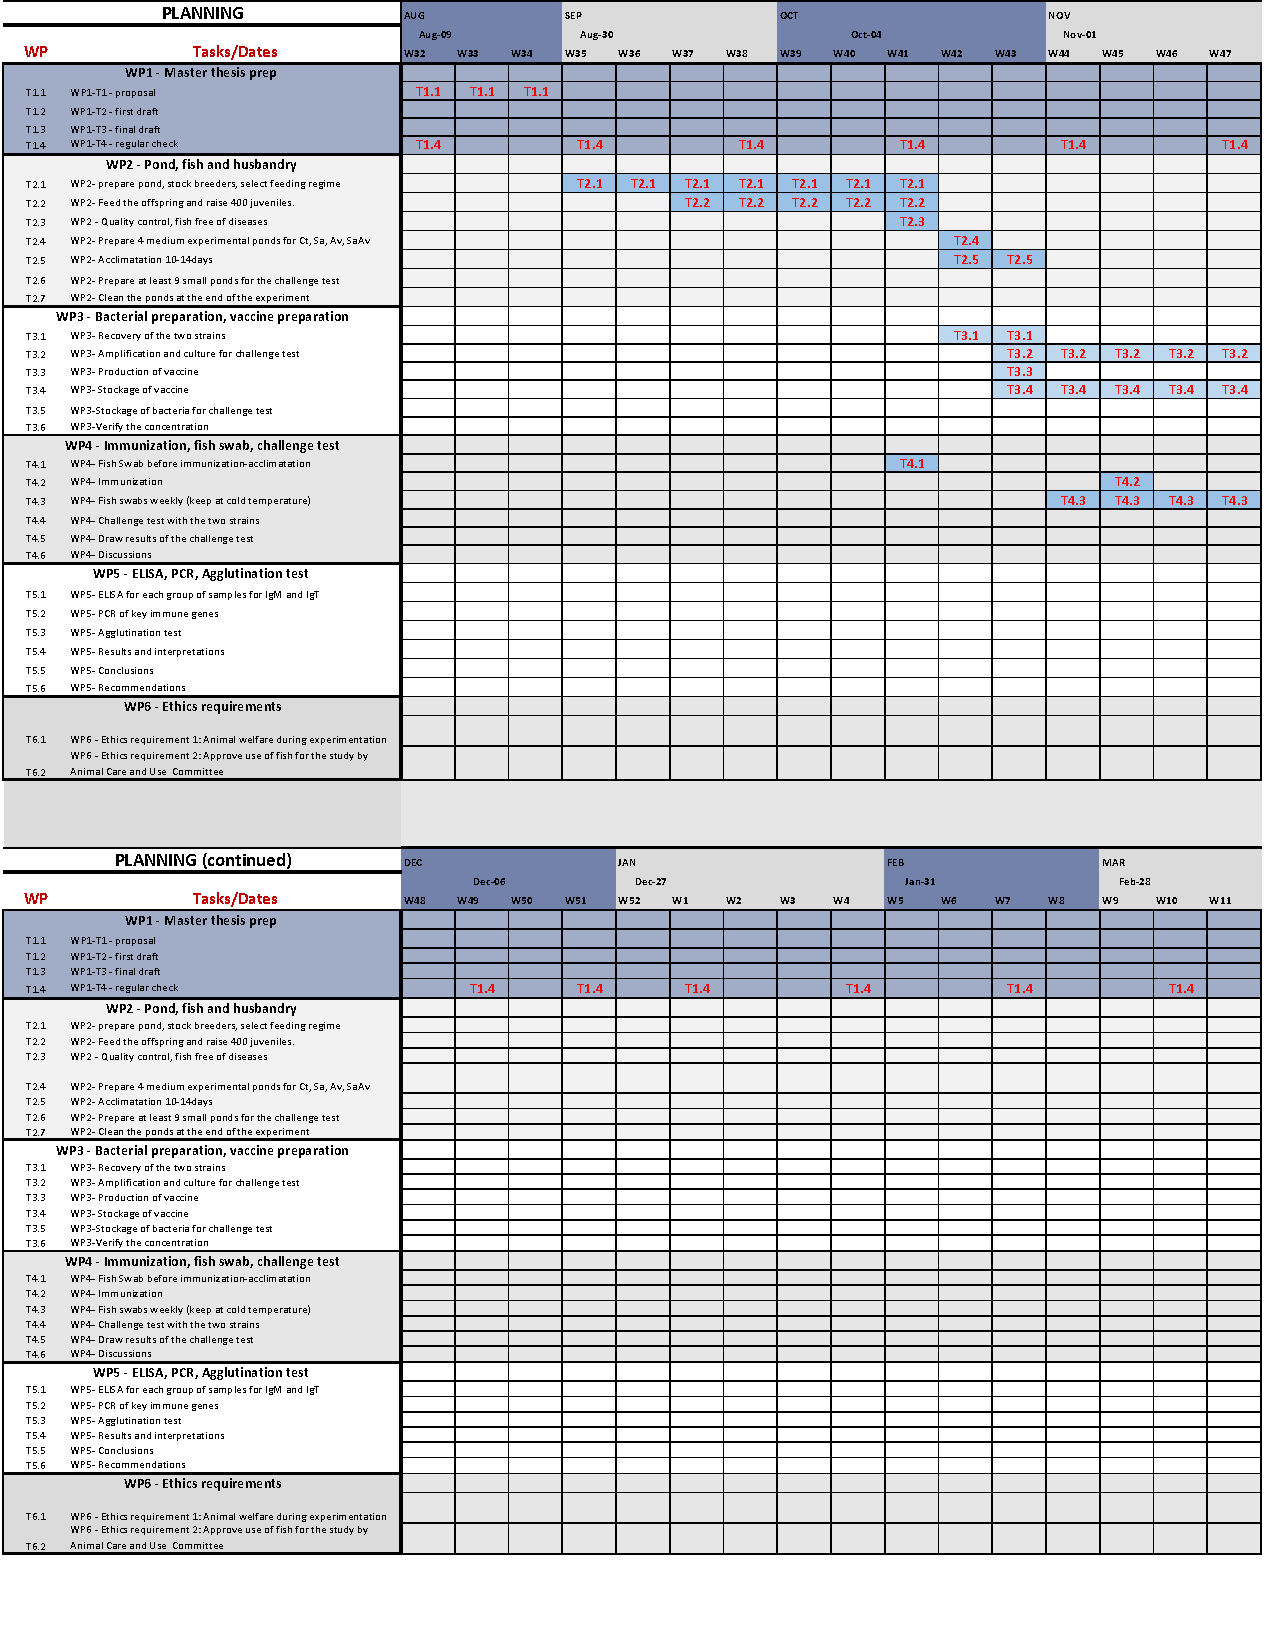
\includegraphics[width=1\textwidth, height=1\textheight, 
                 keepaspectratio]{figures/Planning.pdf}
  \label{Planning august 2021 - march 2022}
  \addcontentsline{lof}{chapter}{Appendice A \hskip 3.55em Planning august 2021 - march 2022}
  \endfigure
  \end{center}
% {\bf Useful documents}
% \beginfigure
%   \begin{flushleft}
%   \caption{\textbf{Planning august-november}}
%   \end{flushleft} 
%   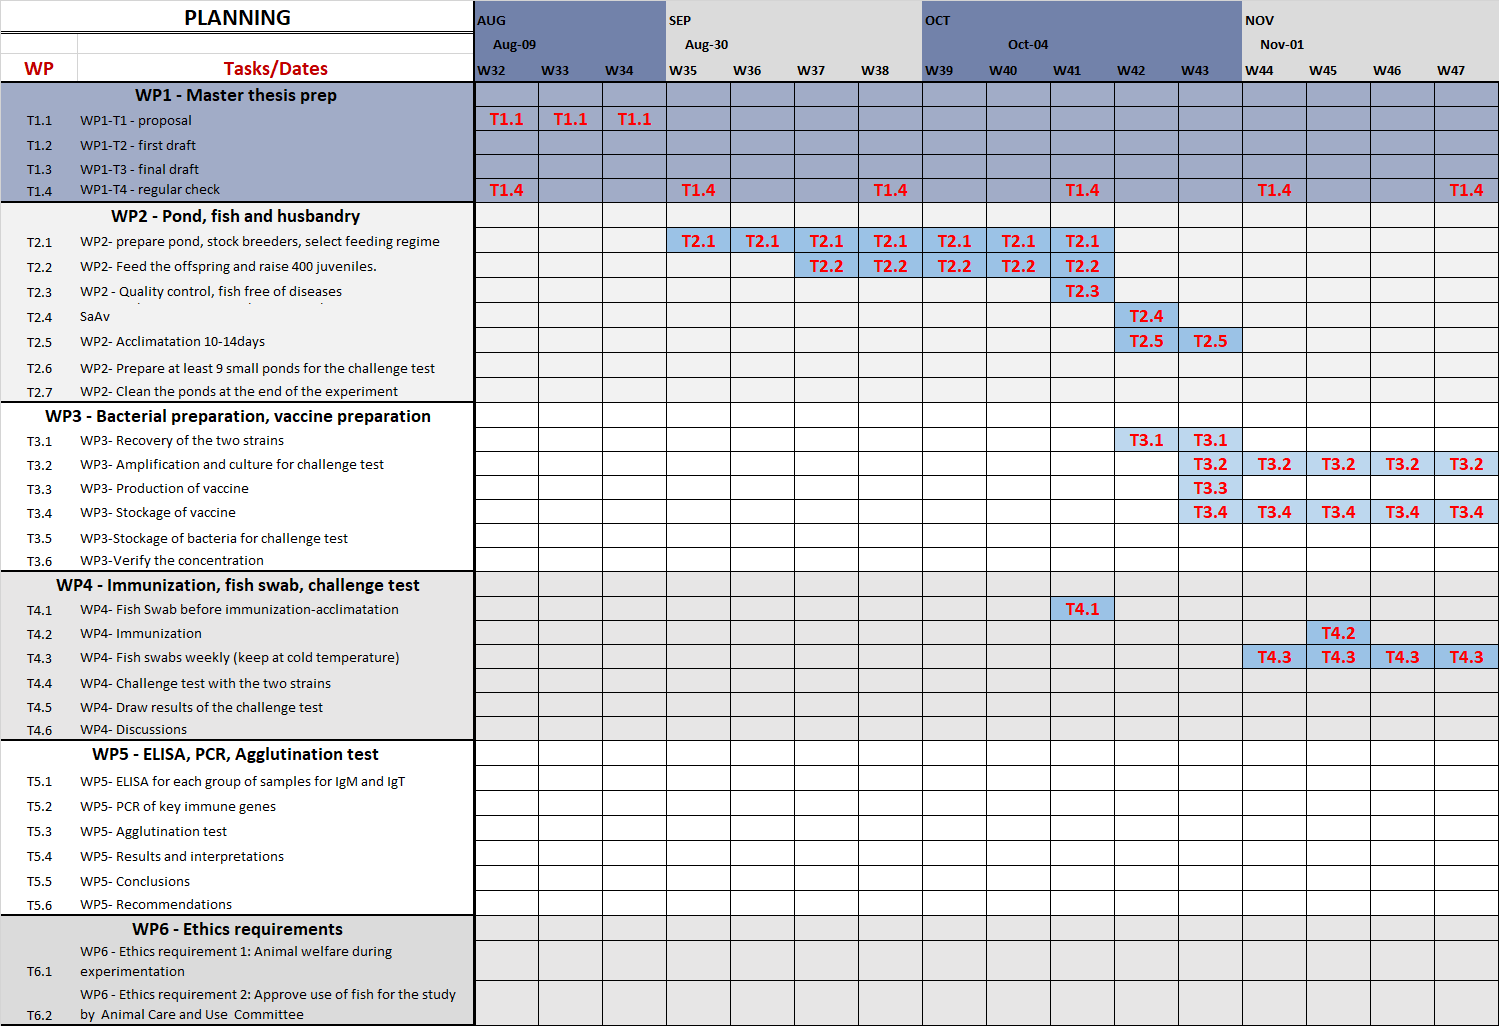
\includegraphics[width=1\textwidth, height=1\textheight, 
%                  keepaspectratio]{figures/Planning1.png}
%   \label{Planning august-november}
%   \addcontentsline{lof}{chapter}{Appendice 1 \hskip 3.55em Planning august-november}
%   \endfigure
% \beginfigure
%   \begin{flushleft}
%   \end{flushleft}
%   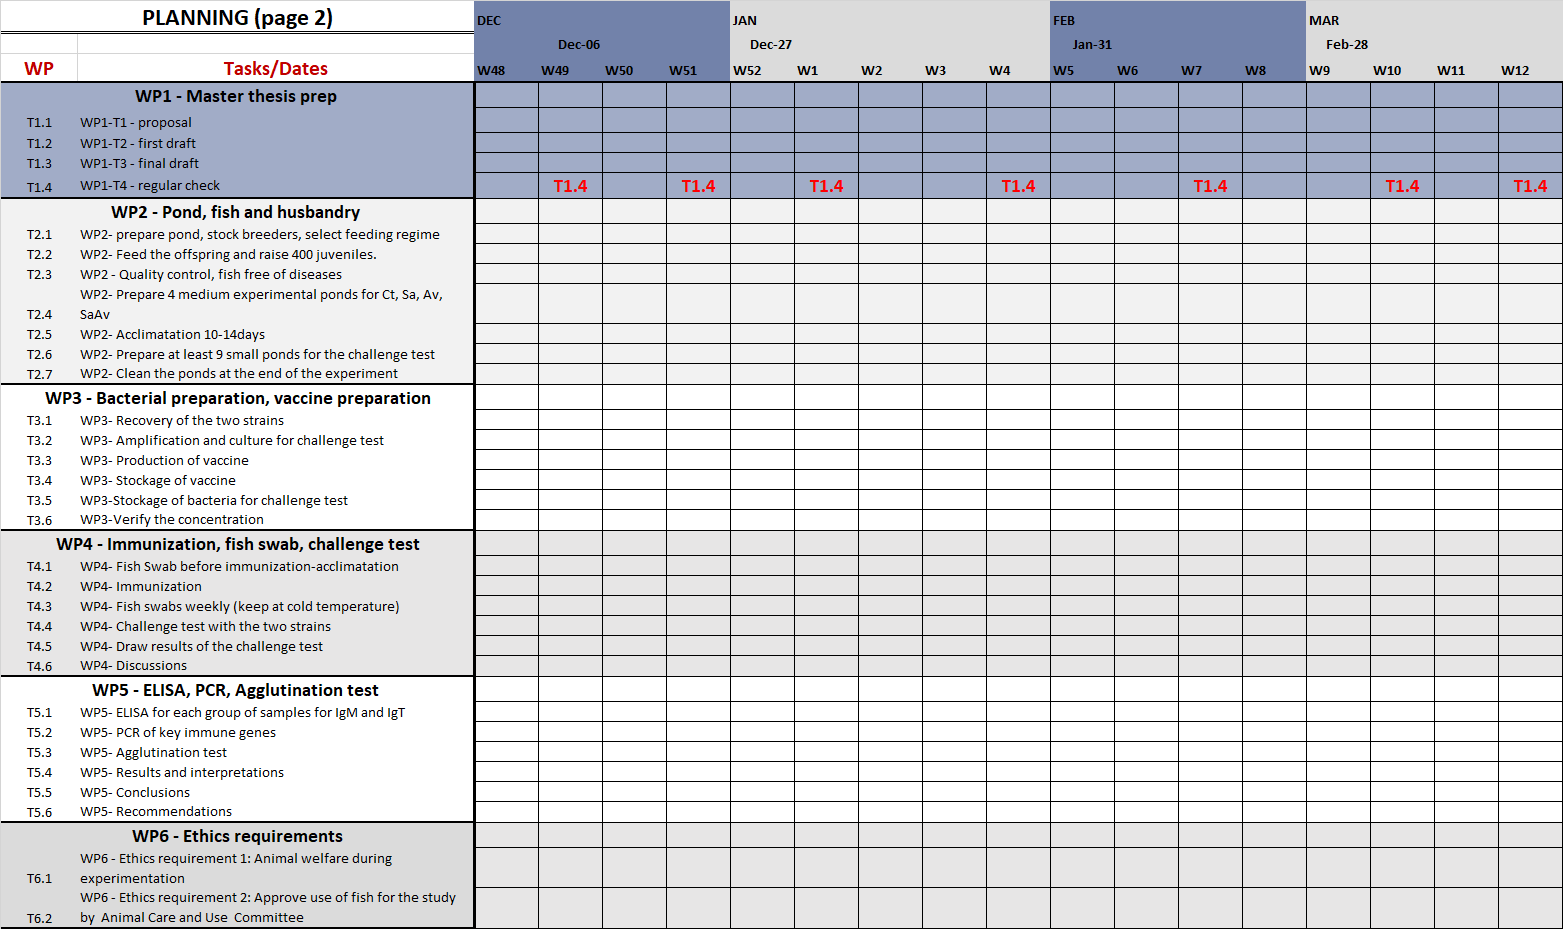
\includegraphics[width=1\textwidth, height=1\textheight, 
%                  keepaspectratio]{figures/Planning2.png}
%   \label{Planning december-march}
%   \addcontentsline{lof}{chapter}{Appendice 2 \hskip 3.55em Planning december-march}
%   \endfigure


\FloatBarrier


\setlength{\footskip}{8mm}

% NOTE: NEED TO DO EVERYTHING SUCH AS SECTION NUMBER OR FIGURE NUMBER 
% MANUALLY IN THIS CHAPTER.

\renewcommand{\thefigure}{A.\arabic{figure}}

\begin{center}
\large \bf APPENDIX B
\vskip 1em
\end{center}

\FloatBarrier

\singlespace
 
{\bf Section Name} \\ 



Some text ..


\FloatBarrier


\addcontentsline{toc}{chapter}{\hskip 3.55em APPENDICES}


\phantomsection
\addcontentsline{toc}{chapter}{\hskip 3.55em VITA}
\setlength{\footskip}{8mm}

% NOTE: NEED TO DO EVERYTHING SUCH AS SECTION NUMBER OR FIGURE NUMBER 
% MANUALLY IN THIS CHAPTER.

\renewcommand{\thefigure}{A.\arabic{figure}}

\begin{center}
\large \bf VITA
\vskip 1em
\end{center}

\FloatBarrier

\singlespace
 
{\bf Section Name} \\ 



Some text ..


\FloatBarrier


\end{document}
